\begin{frame}{Area Between Two Curves}
\begin{center}
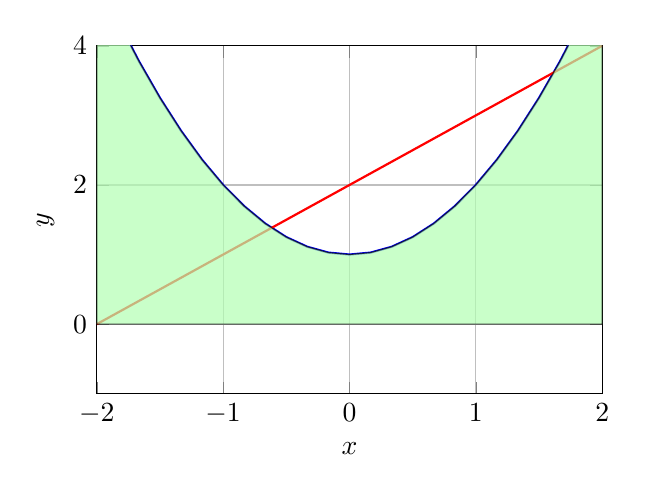
\begin{tikzpicture}
\begin{axis}[
    xlabel={$x$},
    ylabel={$y$},
    grid=both,
    xmin=-2, xmax=2,
    ymin=-1, ymax=4,
    width=8cm,
    height=6cm
]
\addplot[thick, blue, domain=-2:2] {x^2 + 1};
\addplot[thick, red, domain=-2:2] {x + 2};
\addplot[fill=green!30, opacity=0.7, domain=-2:2] {x^2 + 1} \closedcycle;
\end{axis}
\end{tikzpicture}
\end{center}

\footnotesize
\texttt{\textbackslash addplot[fill=green!30, opacity=0.7] fill between[of=A and B];}
\end{frame}